\htwo{Optical Character Recognition}
\sectionauthor{Julian Kusternigg}

\hthree{Allgemeines}

Wie der Name schon sagt, ist "Optical Character Recognition", kurz OCR, eine Technik um aus Bildern oder anderen Dokumentformaten (z.B.: PDF) Zeichen herauszulesen und somit in Text umzuwandeln. Diesen Text kann der Computer dann für weitere Anwendungen verwenden. Dabei ist egal ob der Text im Bild in Druckschrift oder Handschrift geschrieben ist. Ein Computer soll jeden Text, unabhängig der Schriftart, erkennen.

\hfour{Anwendung}

Schon 1914 wurden erste Schritte gemacht, um Zeichen einzulesen. Das "Optophone" ist ein Gerät welches eingelesene Zeichen in damit definierte Töne umwandelt.

1974 forschte Ray Kurzweil an einer OCR Technik die jeden Gedruckten Text, unabhängig der Schriftart, erkennt. Kurzweil entwickelte eine Maschine für Blinde oder Andere, die nicht lesen konnten, indem der eingelesene Text von der Maschine vorgelesen wird.

Heutzutage gibt es viele Anwendungen für die OCR Technologie. Zum Beispiel wird diese verwendet bei Projekt Gutenberg, eine der ältesten Digitalbibliotheken, um Bücher automatisch digitalisieren zu lassen. Aber auch im normalen Alltag stößt man öfters auf Texterkennung. So bietet zum Beispiel Google, bei ihrem Übersetzer, die Möglichkeit in Echtzeit über die Smartphone-Kamera Text übersetzten zu lassen. Auch zum Einlesen von Informationen von z.B.: einem Reisepass wird Zeichenerkennung verwendet, um das mühsame Abschreiben zu vermeiden.

\hfour{Funktionalität}

Bevor man Text aus einem Bild auslesen kann, wird das Bild meist vereinfacht. Es wird dabei das gesamte Bild auf 2 Farben komprimiert, welche helfen sollen Text oder kein Text zu erkennen. Oft wird auch probiert das Bild zusammenzuschneiden so, dass nur mehr der wichtigste Teil mit Text vorhanden ist. Der letzte Schritt gemacht wird ist das Einteilen der Zeichen. Dabei wird probiert alles was ein Zeichen sein könnte zu finden und auszuschneiden.

Diese Bilder von Zeichen werden dann probiert in den jeweiligen Zeichencode
umzuwandeln. Es gibt 2 Herangehensweisen, die meist verwendet werden, um die Umwandlung durchzuführen.

\hfour{Matrix oder Pattern Matching}

Bei diesem Vorgang wird eines der zusammengeschnittenen Zeichenbilder Pixel für Pixel verglichen mit vorgefertigten Zeichen. Anhand von den Prozent, die übereinstimmen kann zurückgeschlossen werden welches Zeichen im Bild sein könnte. Diese Möglichkeit ist recht einfach im Vergleich zur zweiten Technik. Ein Nachteil ist aber das verschiedene Schriftarten problematisch sein könnten und manche Zeichen falsch oder gar nicht erkannt werden. Beheben kann man dieses Problem, indem man die vorgefertigten Zeichen mit denen verglichen wird, erweitert. Das macht den ganzen Vorgang aber wiederum langsamer. Somit muss das Vorgehen für jede Anwendung individuell angepasst werden.

\hfour{Feature Extraction}

Hier wird, wie der Name schon sagt, nach Merkmalen gesucht. Merkmale sind sowas wie Kanten und Kurven also dinge die man braucht, um Zeichen zu beschreiben. Also werden die Merkmale eines Zeichens, welches aus dem Bild geschnitten wurde, verglichen mit einer Ansammlung von typischen Zeichenmerkmalen. Somit kann erkannt werden um welches Symbol es sich handeln könnte. Dieser Vorgang funktioniert oft besser mit verschieden Schriftarten, da nicht auf einen exakten Verglich geschaut wird.

Heutzutage werden auch oft andere Ansätze verwendet, oder sogar eine Mischung aus den Obigen mit Techniken mit neuen Wegen. So extrahieren viele OCR Anbieter zuerst Merkmale von den Zeichen mit Bildern und ein Neurales Netz prüft dann welches Zeichen, das sein könnte.

Oft wird auch nicht nur nach Zeichen gesucht. Gerade bei Sprachen, die mit Leerzeichen getrennt wurden wird probiert ganze Wörter zu finden die dann wieder in Zeichen zu zerlegen, aber trotzdem die fertigen Zeichen mit einem Wörterbuch zu vergleichen, ob das Ergebnis stimmen könnte.

\hfour{Tesseract}

Tesseract ist eine Software aus 1985, die 2005 als Open-Source-Projekt veröffentlicht wurde. Seit 2006 wird das Projekt von Google unterstützt und ist eine der bekanntesten "Optical-Character-Recognition" Software. Zusätzlich zu den oben genannten Arten der Zeichenerkennung, verwendet Tesseract ein Neurales Netz, um die Auswahl noch weiter einzuschließen. Außerdem probiert Tesseract ganze Wörter zu finden die sich aus den Zeichen ergeben könnten, um noch genauere Ergebnisse zu liefern.\cite{OCRIntro}

\hthree{Implementierung}

\hfour{OCR-Modul}

Man kann eine Raumnummer, wie schon beschrieben, nicht nur eingeben, sondern auch mit der Kamera eines Smartphones einscannen. Um die Raumnummer aus den Bildern auszulesen brauchen wird somit OCR. Dabei wird die Bibliothek "TesseractJS" die eine Web-Version von "Tesseract OCR" ist, direkt im Browser eingebunden, um die Bilder von Raumnummern zu Text zu verarbeiten.

Um das eben Erwähnte umzusetzten, gibt es bei ZELIA eine Komponete im Komponentensystem, welche genau diese Funktionalität bewerkstelligt. Diese Komponente wird auf der OCR-Seite des Frontends eingebunden. Sie beinhaltet ein Videoelement um zu zeigen was sie scannt. Um auf die Kamera eines Gerätes aus einem Webbrowser zugreifen zu können, muss über den "Browser Navigator" angefragt ob die Kamera verwendet werden darf.

\typescript{code/OCR/nav.ts}{Zugriff auf eine Kamera im Browser}

Als Parameter, bei dieser Anfrage, kann man defineren worauf man Zugriff haben möchte. Im Falle von ZELIA wird als Videoquelle die Außenkamera angefragt und Audio wird verworfen, da es nicht notwendig ist. Die Browser bestimmen dann ob die Anfrage erlaubt werden soll oder fragen die Benutzer*innen des Gerätes. Wenn der Zugriff abgelehnt wurde, wird das Videoelement, welches die Kamera anzeigen soll, ersetzt duch eine Fehlermeldung. Bekommt der Browser aber die Videoquelle, so zeigt er sie an und startet das "OCR"-Modul.

Die Aufgabe des "OCR"-Moduls ist es Bilder in Text umzuwandeln. Dabei wird TesseractJS verwendet um den "Optiacal Character Recognition" Prozess durchzuführen. Unsere Wahl fiel auf Tesseract da wir am Anfang mit einer einfach verwendbaren Bibliothek testen wollten, ob OCR in unserem Fall gut funktioniert. Da es sehr gute Ergebnisse geliefert hat, wurde es weiterverwendet und ein bisschen optimiert.

\typescript{code/OCR/OCRModule.ts}{Die Verwendeung von TesseractJS}

TesseractJS verwendet sogennante "Worker" um Text aus einem Bild zu extrahieren und je mehr davon vorhanden sind desto schneller geht der Prozess. Nartürlch wird dadurch mehr Prozessorleitung verwendet, was auf Smartphones schnell zu einem erhöhten Energieverbrauch oder erhitzen des Gerätes führt. Somit wird bei ZELIA oft nur ein "Worker" verwendet. Da das initzialisiern dieser services recht lange dauert, gäbe es die möglichkeit mehrere gleichzeitig zu laden. Bei nur einem "Worker" macht das keinen Unterschied, aber wenn man mehrere initzialisiern würde, kann diese Optimirung viel Zeit einsparen.

Zusätzlich um den eingentlichen Umwandlungsvorgang von Bild zu Text zu beschleunigen wird eine Bildoptimierung für OCR durchgeführt. Bevor Tesseract dem Bild die Zeichen entzieht, wird es somit auf ein Schwarz-Weiß-Bild umgewandelt und nur auf den wichtigen Teil, dort wo nichts schwarz ist, zusammengeschnitten. 

Mit diesen Optimierungen liefert Tesseract sehr gute Ergebnisse und somit haben wir die Open-Source Bibliothek weiterverwendet.

\typescript{code/OCR/compress.ts}{Bild vereinfachen bevor Text extrahiert wird}

\begin{figure}
    \centering
    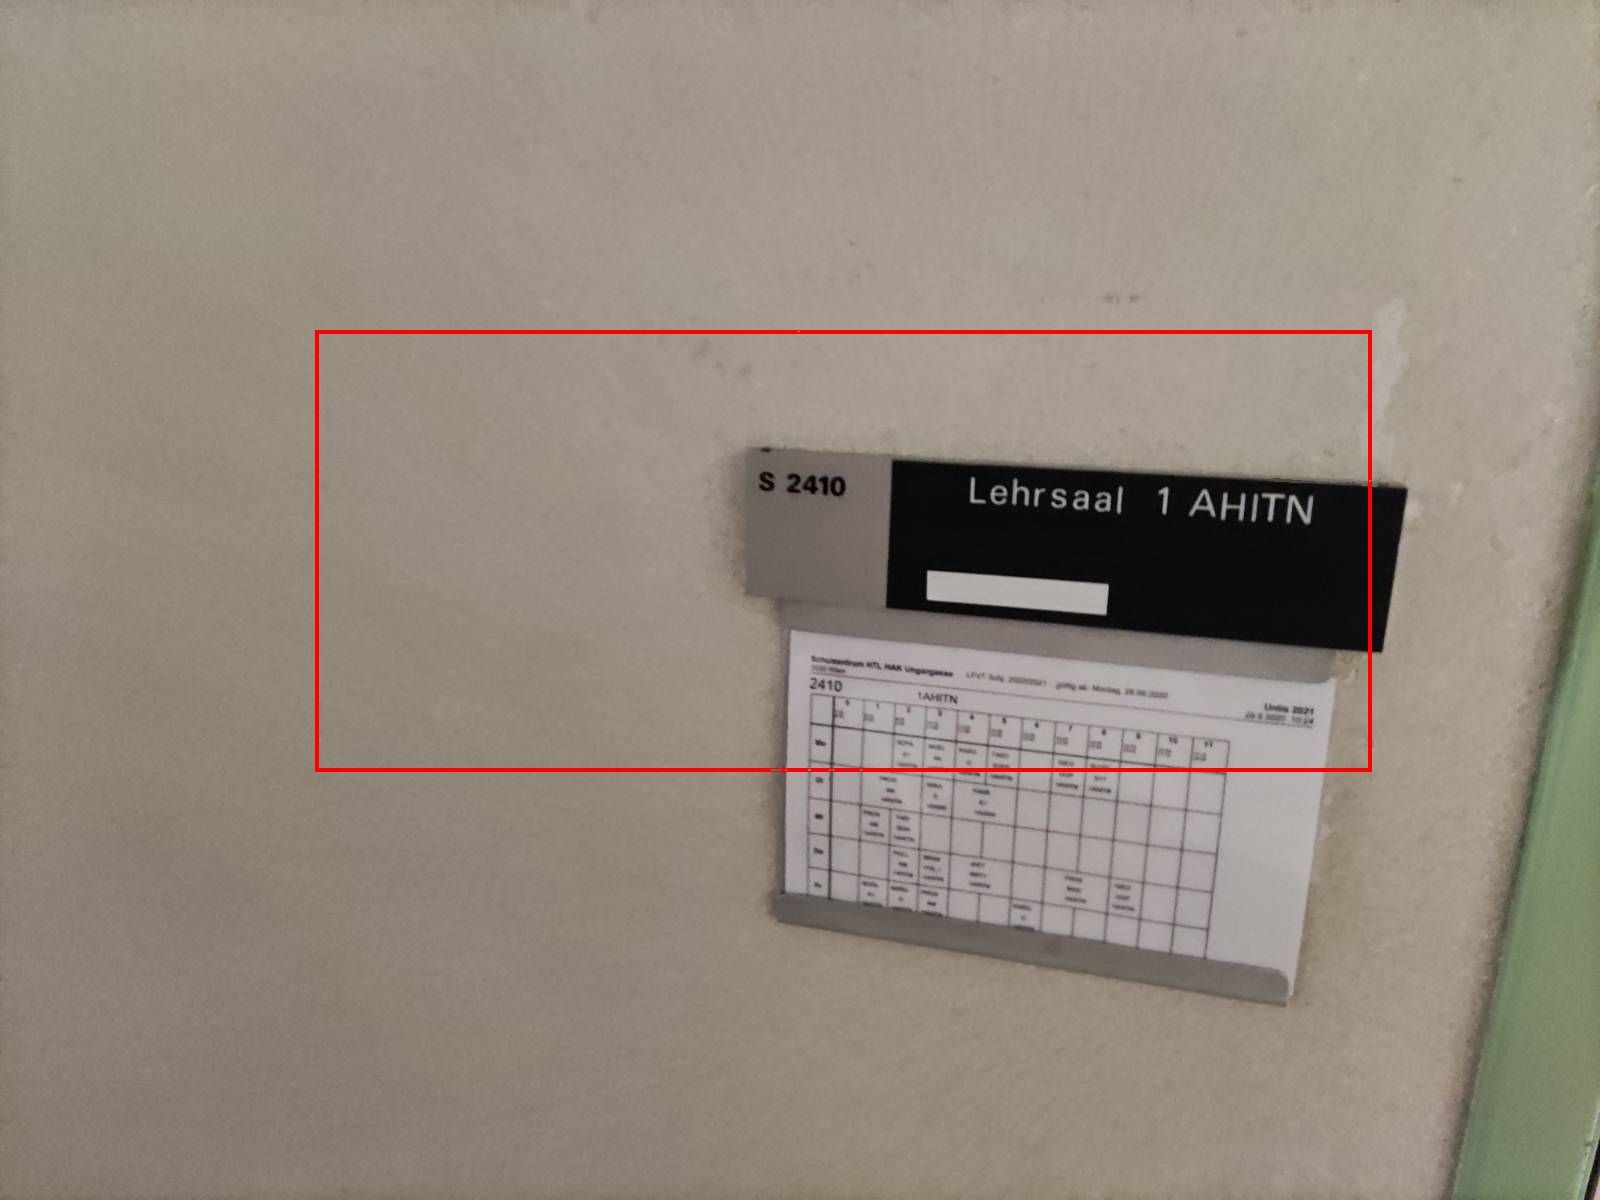
\includegraphics[width=120mm]{media/OCR/original}
    \caption{Aufnahme einer Smartphonekamera (Fokusbereich rot markiert)}
\end{figure}


\begin{figure}
    \centering
    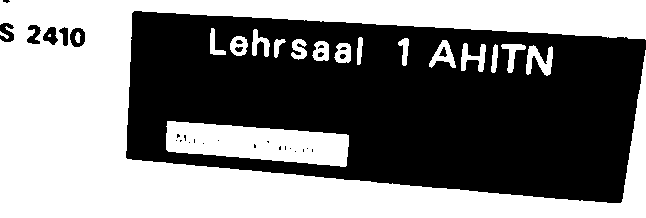
\includegraphics[width=120mm]{media/OCR/compressed}
    \caption{Bild nachdem es für OCR vereinfacht wurde}
\end{figure}

% TODO: Diagnostics (wie schnell ist der Spaß :) )